\documentclass{article}

\usepackage[margin=1in]{geometry}
\usepackage{amssymb}
\usepackage{amsmath}
\usepackage{indentfirst}
\usepackage{algorithm}
\usepackage[noend]{algpseudocode}
\usepackage{underscore}
\usepackage{placeins}
\usepackage{graphicx}
\usepackage{mathrsfs}

\begin{document}

\title{CSCI 6100 \protect\\ OLA3 \protect\\ 0/1 Knapsack Problem}
\author{Cruz Jean}
\maketitle

\section{Problem}
In the 0/1 knapsack problem, we're given a set $S$ of items, each with a weight $S_w \ge 0$ and value $S_v \ge 0$.
Additionally, we're given a knapsack with a weight capacity of $W$.
Our goal is to maximize the total value of all the items we put into the knapsack without going over the weight limit.

Formally, where $X$ denotes the solution:
\begin{align}
X = \max_{value} \left\{x \subseteq S \enspace \bigg| \enspace \sum_{i \in x}{i_w} \leq W\right\}
\end{align}

\pagebreak
\section{Dynamic Programming Solution}

\textbf{Problem:}
Solve the 0/1 knapsack problem via a dynamic programming approach.
This solution constructs a table where each row considers taking or not taking a single item and each column represents a given weight capacity for the knapsack.

\textbf{Inputs:} The set of items and the maximum weight of the knapsack.

\textbf{Outputs:} The solution items, their total weight, and their total value.

\FloatBarrier
\begin{algorithm}
\caption{Dynamic Programming Solution}
\begin{algorithmic}[1]
\Function{Dynamic}{$items, maxweight$}
	\If{$len(items) = 0 \texttt{ or } maxweight \leq 0$}
		\Return $(), 0, 0$
	\EndIf

	\State $table \gets matrix(len(items), maxweight + 1)$
	\State $best \gets ()$
	
	\For {$i = 0 \texttt{ ; } i < items[0].w \texttt{ and } i \leq maxweight \texttt{ ; } \texttt{++}i$}
		\State $table[0, i] \gets 0$
	\EndFor
	\For {$i = items[0].w \texttt{ ; } i \leq maxweight \texttt{ ; } \texttt{++}i$}
		\State $table[0, i] \gets items[0].v$
	\EndFor
	\For {$row = 1 \texttt{ ; } row < len(items) \texttt{ ; } \texttt{++}row$}
		\For {$w = 0 \texttt{ ; } w < items[row].w \texttt{ and } w \leq maxweight \texttt{ ; } \texttt{++}w$}
			\State $table[row, w] \gets table[row-1, w]$
		\EndFor
		\For {$w = items[row].w \texttt{ ; } w \leq maxweight \texttt{ ; } \texttt{++}w$}
			\State $take \gets table[row-1, w-items[row].w] + items[row].v$
			\State $notake \gets table[row-1, w]$
			\State $table[row, w] \gets \max(take, notake)$
		\EndFor
	\EndFor

	\State $w \gets maxweight$
	\For {$i = len(items) \texttt{ ; } \texttt{--}i \texttt{ ; }$}
		\If {$table[i, w] \neq table[i-1,w]$}
			\State $best \gets (best..., i)$
			\State $w \gets w - items[i].w$
		\EndIf
	\EndFor
	\If {$table[i, w] \neq 0$}
		\State $best \gets (best..., 0)$
	\EndIf

	\Return $reversed(best), maxweight - w, table[len(items) - 1, maxweight]$
\EndFunction
\end{algorithmic}
\end{algorithm}
\FloatBarrier

\textbf{Theoretical Every Case Analysis:}
Using this approach, the time complexity depends only on the number of items under consideration and the maximum weight the knapsack can hold.
Thus, this algorithm is invarient of the actual items under consideration and therefore has a trivial every case analysis.

From the above algorithm, we see that it begins by iterating over every position in the table to build up the subproblem solutions.
After this, it iterates over every row in the table to determine the final solution set.
Thus, where $n$ is the number of items under consideration and $w$ is the maximum weight capacity of the knapsack, the every case complexity is simply:
\begin{align}
T(n, w) = \sum_{i=1}^n{\sum_{j=0}^w{1}} + \sum_{i=1}^n{1} &= n(w+1) + n \\
&= n(w + 2) \in \mathcal{O}(nm)
\end{align}

\pagebreak
\section{Backtracking Solution}

\textbf{Problem:}
Solve the 0/1 knapsack problem via a backtracking approach.
This solution iterates over every valid combination of items and takes the one that results in the highest value.

\textbf{Inputs:}
The set of items and the maximum weight of the knapsack.

\textbf{Outputs:}
The solution items, their total weight, and their total value.

\FloatBarrier
\begin{algorithm}
\caption{Backtracking Solution}
\begin{algorithmic}[1]
\Function{Backtracking}{$items, maxweight$}
	\State $queue \gets priorityqueue()$
	\State $best \gets (0, (), 0, 0)$
	\State $queue.add(best)$

	\While {$\texttt{not } empty(queue)$}
		\State $top \gets pop(queue)$

		\If {$top.depth < len(items)$}
			\State $n \gets copy(top)$
			\State $n.depth \gets n.depth + 1$
			\State $queue.add(n)$

			\If {$top.w + items[top.depth].w \leq maxweight$}
				\State $n \gets copy(top)$
				\State $n.depth \gets n.depth + 1$
				\State $n.w \gets n.w + items[top.depth].w$
				\State $n.v \gets n.v + items[top.depth].v$
				\State $n.items \gets (n.items..., top.depth)$
				\State $queue.add(n)$
			\EndIf
		\Else
			\If {$top.v > best.v$}
				\State $best \gets top$
			\EndIf
		\EndIf
	\EndWhile

	\Return $best.items, best.weight, best.value$
\EndFunction
\end{algorithmic}
\end{algorithm}
\FloatBarrier

\textbf{Theoretical Best Case Analysis:}
With this approach, we always generate at least one child for every non-terminal node.
However, we only generate the second child for nodes which have enough weight remaining to hold the given item.
Thus, the best case scenario is when the knapsack is not large enough to contain any of the items.
In this case, we simply iterate through all the items.

Thus, where $n$ is the number of items under consideration and $w$ is the maximum weight capacity of the knapsack, the best case complexity is simply:
\begin{align}
B(n, w) = \sum_{i=1}^n{1} = n \in \mathcal{O}(n)
\end{align}

So in the best case, this algorithm is very efficient.
Indeed, even more efficient than the dynamic programming solution in the best case.

\textbf{Theoretical Worst Case Analysis:}
Similarly, the worst case for this algorithm is created by having the knapsack capacity such that it can contain all of the items simultaneously.
In this case, we must iterate over every combination of the items.

Thus, where $n$ is the number of items under consideration and $w$ is the maximum weight capacity of the knapsack, the worst case complexity is given by:
\begin{align}
W(n, w) = |\mathscr{P}(S)| = 2^n \in \mathcal{O}(2^n)
\end{align}

And we see that in the worst case this approach is very slow if there are a large number of items under consideration (exponential time).

\pagebreak
\section{Branch and Bound Solution}

\textbf{Problem:}
Solve the 0/1 knapsack problem via a branch and bound approach.
This solution is similar to the backtracking approach except that we additionally compute an upper bound for any given partial subset of the items and use it to prune the search tree.
The upper bound applies a greedy algorithm that is allowed to take fractions of any given item.

\textbf{Inputs:}
The set of items and the maximum weight of the knapsack.

\textbf{Outputs:}
The solution items, their total weight, and their total value.

\FloatBarrier
\begin{algorithm}
\caption{Backtracking Solution}
\begin{algorithmic}[1]
\Function{Backtracking}{$items, maxweight$}
	\State $densities \gets ((items, 0)...)$
	\For {$i = 0 \texttt{ ; } i < len(items) \texttt{ ; } \texttt{++}i$}
		\State $densities[i].density \gets items[i].v / items[i].w$
	\EndFor
	\State $sort(densities : density, desc)$
	\State $queue \gets priorityqueue()$
	\State $best \gets (0, (), 0, 0)$
	\State $queue.add(best)$

	\While {$\texttt{not } empty(queue)$}
		\State $top \gets pop(queue)$

		\If {$top.depth < len(items)$}
			\State $n \gets copy(top)$
			\State $n.depth \gets n.depth + 1$
			\If {$\Call{UpperBound}{densities, n, maxweight} > best.v$}
				\State $queue.add(n)$
			\EndIf

			\If {$top.w + items[top.depth].w \leq maxweight$}
				\State $n \gets copy(top)$
				\State $n.depth \gets n.depth + 1$
				\State $n.w \gets n.w + items[top.depth].w$
				\State $n.v \gets n.v + items[top.depth].v$
				\State $n.items \gets (n.items..., top.depth)$
				\If {$\Call{UpperBound}{densities, n, maxweight} > best.v$}
					\State $queue.add(n)$
				\EndIf
			\EndIf
		\Else
			\If {$top.v > best.v$}
				\State $best \gets top$
			\EndIf
		\EndIf
	\EndWhile

	\Return $best.items, best.weight, best.value$
\EndFunction
\end{algorithmic}
\end{algorithm}
\FloatBarrier

\FloatBarrier
\begin{algorithm}[h!]
\caption{Backtracking Solution - Upper Bound}
\begin{algorithmic}[1]
\Function{UpperBound}{$densities, node, maxweight$}
	\State $w \gets node.w$
	\State $value \gets node.v$

	\For{$i node.depth \texttt{ ; } i < len(densities) \texttt{ ; } \texttt{++}i$}
		\If {$w + densities[i].item.w \leq maxweight$}
			\State $w \gets w + densities[i].item.w$
			\State $value \gets value + densities[i].item.v$
		\Else
			\State $value \gets value + (maxweight - w) * densities[i].density$
			\State $\texttt{break}$
		\EndIf
	\EndFor

	\Return $value$
\EndFunction
\end{algorithmic}
\end{algorithm}
\FloatBarrier

\pagebreak
\textbf{Theoretical Best Case Analysis:}
The only difference between this algorithm and the branch and bound approach is the use of an additional property of a search node (i.e. upper bound) to further prune the search space.
However, this only helps in the average case.
Thus, the best case for this algorithm is the same as the best case for the branch and bound solution:
\begin{align}
B(n, w) = \sum_{i=1}^n{1} = n \in \mathcal{O}(n)
\end{align}

\textbf{Theoretical Worst Case Analysis:}
Similarly, the worst case for this algorithm is the same as the worst case for the branch and bound solution:
\begin{align}
W(n, w) = |\mathscr{P}(S)| = 2^n \in \mathcal{O}(2^n)
\end{align}

\textbf{Average Case:}
From the above, we see that the theoretical best and worst cases for this approach are identical to the backtracking solution.
If we were to perform the average case analysis, we would likewise see that the theoretical average case performance is nearly identical.
However, this is only because we're performing our theoretical analysis in all generality, making no assumptions about the nature of the items under consideration or the capacity of the knapsack.
When these factors are taken into account, the additional pruning of this algorithm is typically faster than the branch and bound algorithm as the problems get larger and larger.

\pagebreak
\section{Experiment}

\textbf{Description:}
The program has a pre-set collection of settings to use for generating several passes of applying each algorithm to a randomly-constructed set of items (weight and value).
These settings are selected not to draw out information about the best/worst case performance of these algorithms, but for the average case.
Because of this, none of the pre-set collections of settings include very large disparities in item weights and max knapsack weight.
Aside from selecting new random values on each pass, the primary factor that will be examined is the time complexity as the number of items under consideration increases.
We will then use this information to hypothesize about the average case efficency of each algorithm as the number of items increases.

Two values will be gathered to analyze the performance of each algorithm.
The first is the number of value comparisons that were made during the runtime of the algorithm.
For any given algorithm, this will necessarily be proportional to the time complexity for different inputs.
However, these algorithms work very differently, and therefore the number of comparisons is perhaps not sufficient to accurately measure the performance differences among these algorithms.
Therefore, the main statistic that will be examined is the runtime of each algorithm in milliseconds.

\textbf{Inputs:}
No user input is taken from the user.
All values are generated randomly at runtime, as per a pre-set collection of settings for each pass.

\textbf{Outputs:}
The only output from this program is the tabulated results from running each pass on each collection of settings.
This information includes the number of items for each pass, the maximum weight, the random weight upper bound, and the random value upper bound.

\textbf{Assumptions:}
No assumptions were made about the number of items under consideration, nor the maximum weight of the knapsack.
Additionally, we made no assumptions of the distribution of the values and weights of each item.
Because of this, any values used in testing would be equally accurate with regards to our theoretical analysis.

\textbf{Random Numbers:}
Random values used in the testing program are high-quality pseudo-random numbers generated by an instance of \texttt{std::mt19937} from the \texttt{<random>} header, which is a 32-bit specialization of Matsumoto and Nishimura's Mersenne Twister algorithm.
The pseudo-random number generator is seeded by an instance of \texttt{std::random_device}, which produces non-deterministic random values (if the system supports this).
The instance of \texttt{std::mt19937} is a uniform bit generator that is used to generate the various types of random distributions used throughout the program.

\section{Experimental Results}

\FloatBarrier
\begin{figure}[!ht]
\centering
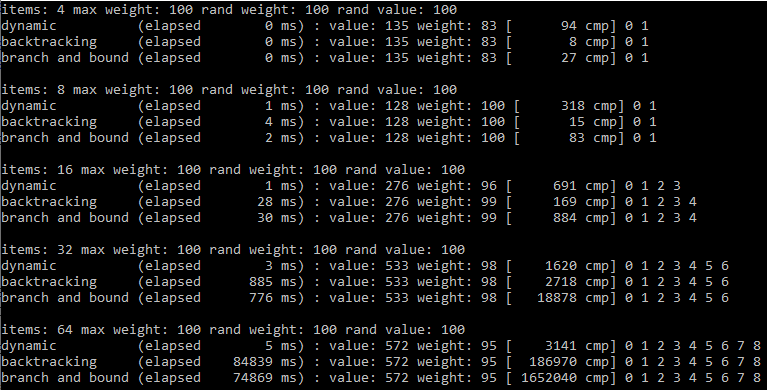
\includegraphics[width=135mm]{output.png}
\caption{Program output used for conclusions}
\end{figure}
\FloatBarrier

\section{Conclusions}

The first thing we notice from examining the program output is that our dynamic programming algorithm clearly has a linear increase in both number of comparisons and elapsed time as the number of items increases.
This is exactly what we would expect given the existence of its every case analysis.

Next, we notice that the branch and bound algorithm is around 12\% faster than the backtracking algorithm for any given run.
This is what we would expect from our theoretical analysis, as the branch and bound approach is able to prune more branches from the search space than the backtracking approach.
However, we also see that the branch and bound approach has significantly more value comparisons than the equivalent backtracking approach.
This is due to the added complexity of generating the upper bound values for every node, and serves as demonstration for why we have selected elapsed time as the primary factor by which to draw comparisons between these significantly-different approaches.

And of course, we see that the rate of increase in runtime with respect to the number of items is significantly worse than linear for both the backtracking and branch and bound approaches.
However they are not as bad as our theoretical worst case.
Indeed, we see that from one pass to the next we double the number of items and the runtime increases by factors of increasing powers of 3.
This would of course mean that we have roughly $A(n,m) \in \mathcal{O}((\frac{3}{2})^n)$ time complexity.
This is of course due to these algorithms using a pruned search tree.

In conclusion, we see that the dynamic programming approach is significantly better than both the backtracking and branch and bound approaches for the test cases used in this analysis.
It should be noted that there are edge cases in which the dynamic programming approach is slower, but the data must practically be tailored specifically to this end, and is therefore not a typical average case.
And so we have that, for a constant size of knapsack, the dynamic programming approach is precisely linear in the number of items under consideration and both other algorithms are exponential with an approximate branching factor of 1.5.
Thus, if performance in the typical, average case is desired, the dynamic programming algorithm should be used.

\end{document}
